\chapter{Auger Decay of Noble Gas Atoms}
The decay widths of noble gas atoms have been thoroughly studied in the
literature. Therefore, the main aim of this chapter is to prove the implementation
of the FanoADC-Stieltjes in the Dirac programme \cite{DIRAC13} to work
reliably and reproduce results known in the literature. Both, the neon atom
and the xenon atom are investigated.
The neon atom is chosen, because reference data is available
obtained from a non-relativistic
implementation of the same method. Then, the xenon atom is studied, due
to the importance of relativistic effects in its description, which is
the focus of this thesis.
Finally, the results will be used to verify that the programme is
able to predict the decay widths of autoionization processes.
In contrast to other comparable relativistic programmes
\cite{Tulkki92,Fritzsche12}, the FanoADC-Stieltjes approach does not
rely on spherical symmetry and is therefore capable of describing
the decay widths of \ac{ICD} processes.


\section{Neon}

The Ne1s$^{-1}$ vacancy with an ionization energy of \unit[870]{eV}
\cite{Saethre84} is
the initial state of the Auger decay. The double ionization energies of
the final states are shown in Table \ref{table:Ne_dips}. Hence, the
kinetic energy of the emitted electron lies between
\unit[748]{eV} and \unit[808]{eV}.

\begin{table}[h]
  \centering
  \caption{Experimental ionization energies of the doubly ionized final states
           \cite{NIST2014}.}
  \begin{tabular}{llr}
   \toprule
   \multicolumn{2}{c}{Final states} & \acs{SIP} [eV]\\
   \midrule
   \multirow{5}{*}{2p$^{-2}$} & $^3P_0$        & 62.52 \\
                              & $^3P_1$        & 62.60 \\
                              & $^3P_2$        & 62.64 \\
                              & $^1D$          & 65.73 \\
                              & $^1S$          & 69.44 \\
   \midrule
 \multirow{4}{*}{2s$^{-1}$2p$^{-1}$} & $^3P_0$ & 87.85 \\
                              & $^3P_1$        & 87.92 \\
                              & $^3P_2$        & 87.96 \\
                              & $^1P$          & 98.41 \\
   \midrule                                    
      2s$^{-2}$               & $^1S$          &121.89 \\
   \bottomrule
  \end{tabular}
  \label{table:Ne_dips}
\end{table}

\subsection{Computational Details}
The decay width calculations were performed using the FanoADC-Stieltjes approach
implemented in the programme package \verb|DIRAC| \cite{DIRAC13}.
A cc-pCV6Z basis set was employed with
additional $s$, $p$ and $d$ functions (5,5,6) of the \ac{KBJ} type \cite{Kaufmann89}.
The active space covered an energy range of \unit[-33.0 -- 56.0]{a.u.}, and included
376 spinors in both, the relativistic and the non-relativistic calculation.

\subsection{Decay Widths}
The calculated decay widths are outlined and compared to experimental
results in Table \ref{table:Ne_gammas}. Hereby, the contributions to the
total decay widths are given
for the three groups 2p$^{-2}$, 2s$^{-1}$2p$^{-1}$ and 2s$^{-2}$ as well
as for the different terms explicitely, as far as numbers are available.

\begin{table}[h]
  \centering
  \caption{Auger decay widths and contributions of the different channels to
           the total decay width in \% 
           for an initial vacancy in the Ne1s. The decay widths are given in
           \unit[]{meV}.}
  \small
  \begin{tabular}{llr|rr|rr|rr|rr|rr}
   \toprule
    & & \multicolumn{3}{c}{This work} & \multicolumn{2}{c}{Koloren\v{c}} & \multicolumn{2}{c}{Kelly} & \multicolumn{2}{c}{Yarzhemsky} & \multicolumn{2}{c}{exp.}\\
   \multicolumn{2}{c}{Final states} & {rel.} & \multicolumn{2}{c|}{nrel.} & \multicolumn{2}{c|}{Ref.\cite{Kolorenc11}} & \multicolumn{2}{c|}{Ref.\cite{Kelly75}} & \multicolumn{2}{c|}{Ref.\cite{Yarzhemsky02}} & \multicolumn{2}{c}{Refs. \cite{Albiez90}, \cite{Avaldi95}}\\
   \midrule
   \multirow{3}{*}{2p$^{-2}$} & $^3P$   & \multirow{3}{*}{53.9} & 0.0 & \multirow{3}{*}{81.6} &  0.0 & \multirow{3}{*}{60.0} &  0.0 & \multirow{3}{*}{70.8} &  0.0 & \multirow{3}{*}{68.4} &  --  & \multirow{3}{*}{70.4}\\
                              & $^1D$      & & \multirow{2}{*}{81.6} & & 50.5 & & 61.2 & & 58.2 & & 60.9&\\
                              & $^1S$      & &  & &  9.5 & &  9.6 & & 10.2 & &  9.5&\\
   \midrule
 \multirow{2}{*}{2s$^{-1}$2p$^{-1}$} & $^3P$     & \multirow{2}{*}{38.0} & 1.1 & \multirow{2}{*}{7.8} & 10.6 & \multirow{2}{*}{30.1} &  6.1 & \multirow{2}{*}{23.1} &  9.3 & \multirow{2}{*}{26.1} &  6.3 & \multirow{2}{*}{23.5}\\
                              & $^1P$ &       &  6.8 & & 19.5 & & 17.0 & & 16.8 & & 17.2&\\
   \midrule
      2s$^{-2}$               & $^1S$ &       8.1 & 10.4 & 10.4 &  9.9 & 9.9 &  6.1 & 6.1 &  5.5 & 5.5 &  6.1& 6.1\\
   \midrule
   $\Gamma$  & & {344}  & \multicolumn{2}{c|}{268} & \multicolumn{2}{c|}{251} & \multicolumn{2}{c|}{219} & \multicolumn{2}{c|}{242} & \multicolumn{2}{c}{220 $\pm$ 30}\\
   \bottomrule
  \end{tabular}
  \label{table:Ne_gammas}
\end{table}

The results of this work were obtained using the FanoADC-Stieltjes method and
the same basis set as in the work of  Koloren\v{c} \textit{et al.}
\cite{Kolorenc11}. However, the latter non-relativistic description uses an
energy based partitioning.
Focussing on the total decay width, the non-relativistic decay width
obtained in this thesis is of the same order of magnitude
as both the experimental result
and the other theoretical predictions, while the relativistic result
overestimates the experimental decay width by \unit[56]{\%}. However, this
discrepancy is still inside the error margins of the FanoADC-Stieltjes method.

The branching ratios obtained from the partial decay widths of the present
results have the correct order of magnitude in the relativistic calculation, but
deviate from the values found in the literature. In the non-relativistic case
the 2s$^{-1}$2p$^{-1}$ channel's contribution is substantially underestimated.
It is known from the literature \cite{Aaberg82} that taking into account
the coupling of the 2s and the 2p orbitals is crucial in order to obtain
reliable values for the decay width. Since this coupling is neglected
in the current projection scheme, these branching ratios cannot be reproduced.
The partial decay width of the 2p$^{-2}$ $^3P$ channel is forbidden by symmetry.
In an Auger decay the angular momentum and the spin need to be conserved
in the Russel-Saunders coupling scheme, i.e. $\Delta L = \Delta S = 0$.
The initial state is characterized by $L_i = 0$, $S_i= \frac12$ and
has $g$ symmetry. The
2p$^{-2}$ $^3P$ final state without the electron is characterized by $L_f=1$
and $S_f = 1$ and is a $g$ state. In order to conserve the momenta, the
outgoing electron would have to be characterized by $L_e=1$ and $S_e=\frac12$.
However, this outgoing electron would have ungerade symmetry. Since the coupling
operator is the gerade Coulomb operator, the corresponding matrix elements
are zero.
This property is correctly predicted by the current implementation of the
FanoADC.




\section{Xenon}
From single and double ionization spectra and Auger spectroscopy
it is known that vacancies from the Xe4d and lower are energetically allowed to
decay via Auger processes. \cite{Siegbahn69}
In the following, I will focus on two energetic initial state regions, namely
the 4p and the 4d region.

\subsection{Computational Details}
All calculations in this chapter, including the decay width calculations,
were performed using the
Dyall cv4z basis set \cite{dyall5p06} with additional five s, p and d
and three diffuse basis functions                       
of the \ac{KBJ} type \cite{Kaufmann89}. The active space was chosen to include the
the fourth shell completely and the positive energies to be limited by
\unit[40.0]{a.u.}.

\subsection{Open Channels}
The different open channels are to be determined by comparison of the single
and double ionization spectra shown in Figure \ref{figure:Xe_sdip}.
These spectra have been calculated using the
DC-ADC(2x) method implemented in \verb|DIRAC|
\cite{Pernpointner04_1,Pernpointner10_1,DIRAC13}.

\begin{figure}[]
  \centering
  \begin{tikzpicture}[scale=1.0]

\begin{axis}[%scale=1.5,
             domain=30:170,
             %y domain=1E-8:10,
             restrict expr to domain={x}{30:170},
             xlabel={E in \unit{eV}},
             xtick={30,50,...,170},
             %xticklabels={2,4,6,8,10,12,15,20,25},
             ytick={-1.0,-0.8,...,1.0},
             yticklabels={1.0,0.8,0.6,0.4,0.2,0.0,0.2,0.4,0.6,0.8,1.0},
             ylabel={pole strength},
             scale only axis,
             width=\textwidth-2cm,
             height=7cm
             %title={Parameter Fitting of NeNe and NeAr Decay Widths}
             ]

\draw[gray]
  (axis cs:\pgfkeysvalueof{/pgfplots/xmin},0) --
  (axis cs:\pgfkeysvalueof{/pgfplots/xmax},0);
\addplot+[ycomb,
         %no markers,
         mark=.,
         thick,
         diplom1,
         forget plot
        ]
        table[
        x expr = \thisrowno{0},
        y expr = \thisrowno{1}
        ]
        {data/Xe_rel_sips.dat};
        \addlegendimage{line legend, diplom1, thick};
        \addlegendentry{SIPs(Xe)};
\addplot+[ycomb,
         %no markers,
         mark=.,
         thick,
         diplom2,
         forget plot
        ]
        table[
        x expr = \thisrowno{0},
        y expr = -\thisrowno{1}
        ]
        {data/Xe_rel_dips.dat};
        \addlegendimage{line legend, diplom2, thick};
        \addlegendentry{DIPs(Xe)};

\node[pin={[pin distance=0.2cm]170:{\tiny 4d$_{5/2}^{-1}$}}]
     at (axis cs:67.03,0.6) {};
\node[pin={[pin distance=0.2cm]10:{\tiny 4d$_{3/2}^{-1}$}}]
     at (axis cs:69.06,0.6) {};
\node[pin={[pin distance=0.2cm]170:{\tiny 4p$_{3/2}^{-1}$}}]
     at (axis cs:146.6,0.2) {};
\draw[] (axis cs:165,0.15) arc [radius=0.75cm,start angle=10,end angle=100];
\node[pin={[pin distance=0.2cm]20:{\tiny 4p$_{1/2}^{-1}$}}]
     at (axis cs:159.6,0.23) {};
 		
%DIPs
\draw[] (axis cs:39,-0.9) arc [radius=0.3cm,start angle=358,end angle=180];
\node[pin={[pin distance=0.10cm]95:{\tiny 5p$^{-2}$}}]
     at (axis cs:32,-0.75) {};

\draw[] (axis cs:50,-0.75) arc [radius=0.3cm,start angle=358,end angle=180];
\node[pin={[pin distance=0.05cm]280:{\tiny 5s$^{-1}$5p$^{-1}$}}]
     at (axis cs:47,-0.80) {};

\node[pin={[pin distance=0.1cm]350:{\tiny 5s$^{-2}$}}]
     at (axis cs:59,-0.35) {};

\draw[] (axis cs:96,-0.80) arc [radius=0.3cm,start angle=358,end angle=180];
\node[pin={[pin distance=0.05cm]270:{\tiny 4d$^{-1}$5p$^{-1}$}}]
     at (axis cs:91,-0.85) {};

\draw[] (axis cs:110,-0.70) arc [radius=0.3cm,start angle=358,end angle=180];
\node[pin={[pin distance=0.05cm]300:{\tiny 4d$^{-1}$5s$^{-1}$}}]
     at (axis cs:106,-0.75) {};

\draw[] (axis cs:165,-0.75) arc [radius=0.65cm,start angle=340,end angle=180];
\node[pin={[pin distance=0.05cm]260:{\tiny 4d$^{-2}$}}]
     at (axis cs:154,-0.80) {};

\end{axis}
\end{tikzpicture}

  \begin{tikzpicture}[scale=1.0]

\begin{axis}[%scale=1.5,
             domain=30:170,
             %y domain=1E-8:10,
             restrict expr to domain={x}{30:170},
             xlabel={E in \unit{eV}},
             xtick={30,50,...,170},
             %xticklabels={2,4,6,8,10,12,15,20,25},
             ytick={-1.0,-0.8,...,1.0},
             yticklabels={1.0,0.8,0.6,0.4,0.2,0.0,0.2,0.4,0.6,0.8,1.0},
             ylabel={pole strength},
             scale only axis,
             width=\textwidth-2cm,
             height=7cm
             %title={Parameter Fitting of NeNe and NeAr Decay Widths}
             ]

\draw[gray]
  (axis cs:\pgfkeysvalueof{/pgfplots/xmin},0) --
  (axis cs:\pgfkeysvalueof{/pgfplots/xmax},0);
\addplot+[ycomb,
         %no markers,
         mark=.,
         thick,
         diplom1,
         empty legend
        ]
        table[
        x expr = \thisrowno{0},
        y expr = \thisrowno{1}
        ]
        {data/Xe_nrel_sips.dat};
        \addlegendentry{SIPs(Xe)};
\addplot+[ycomb,
         %no markers,
         mark=.,
         thick,
         diplom2,
         empty legend
        ]
        table[
        x expr = \thisrowno{0},
        y expr = -\thisrowno{1}
        ]
        {data/Xe_nrel_dips.dat};
        \addlegendentry{DIPs(Xe)};

\node[pin={[pin distance=0.2cm]10:{\tiny 4d$^{-1}$}}]
     at (axis cs:69.06,0.6) {};
\draw[] (axis cs:155,0.41) arc [radius=0.5cm,start angle=10,end angle=100];
\node[pin={[pin distance=0.2cm]20:{\tiny 4p$^{-1}$}}]
     at (axis cs:152.0,0.43) {};
 		
%DIPs
\draw[] (axis cs:39,-0.9) arc [radius=0.2cm,start angle=358,end angle=180];
\node[pin={[pin distance=0.1cm]95:{\tiny 5p$^{-2}$}}]
     at (axis cs:32,-0.75) {};

\draw[] (axis cs:50,-0.70) arc [radius=0.2cm,start angle=358,end angle=180];
\node[pin={[pin distance=0.05cm]280:{\tiny 5s$^{-1}$5p$^{-1}$}}]
     at (axis cs:47,-0.75) {};

\node[pin={[pin distance=0.1cm]350:{\tiny 5s$^{-2}$}}]
     at (axis cs:55,-0.40) {};

\draw[] (axis cs:100,-0.80) arc [radius=0.22cm,start angle=358,end angle=180];
\node[pin={[pin distance=0.05cm]270:{\tiny 4d$^{-1}$5p$^{-1}$}}]
     at (axis cs:94,-0.85) {};

\draw[] (axis cs:111,-0.70) arc [radius=0.22cm,start angle=358,end angle=180];
\node[pin={[pin distance=0.05cm]300:{\tiny 4d$^{-1}$5s$^{-1}$}}]
     at (axis cs:107,-0.75) {};

\draw[] (axis cs:170,-0.75) arc [radius=0.45cm,start angle=340,end angle=180];
\node[pin={[pin distance=0.05cm]260:{\tiny 4d$^{-2}$}}]
     at (axis cs:156,-0.80) {};

\end{axis}
\end{tikzpicture}

  \caption{Comparison of calculated single and double ionization spectra
           for the determination of open channels in of the later decay
           width calculation. Upper panel: relativistic description, lower
           panel: non-relativistic description.
           }
  \label{figure:Xe_sdip}
\end{figure}
%\afterpage{\clearpage}


From the calculated single and double ionization spectra the open channels
for different singly ionized initial states can be determined as shown in 
Table \ref{table:Xe_open_channels} and doubly ionized final states.
These results are the basis for the choice of the final state subspace
in the decay width calculations.
\begin{table}[h]
  \centering
  \caption{Channels of the Auger processes for different singly ionized
           initial states and doubly ionized final states
           of the xenon atom. Open channels are marked by "x", while closed
           channels are marked by "--".}
  \begin{tabular}{lcccccc}
   \toprule
                   & 4d$^{-2}$ & 4d$^{-1}$5s$^{-1}$ & 4d$^{-1}$5p$^{-1}$ & 5s$^{-2}$ & 5s$^{-1}$5p$^{-1}$ & 5p$^{-2}$ \\
   \midrule
   4d$_{5/2}^{-1}$ &      --   &       --           &        --          &     x     &     x              &     x     \\
   4d$_{3/2}^{-1}$ &      --   &       --           &        --          &     x     &     x              &     x     \\
   4p$_{3/2}^{-1}$ &      --   &        x           &         x          &     x     &     x              &     x     \\
   4p$_{1/2}^{-1}$ &       x   &        x           &         x          &     x     &     x              &     x     \\
   \midrule
   4d$^{-1}_{nrel}$&      --   &       --           &        --          &     x     &     x              &     x     \\
   %4p$^{-1}_{nrel}$&      --   &        x           &         x          &     x     &     x              &     x     \\
   \bottomrule
  \end{tabular}
  \label{table:Xe_open_channels}
\end{table}




\subsection{Auger Decay from the Xe4d Region}

The Auger process from the Xe4d subshell has been experimentally
measured to high accuracy \cite{Carroll02} and is used as a calibration standard.
The corresponding decay widths have among others been measured by Ausmees
\textit{et al.} \cite{Ausmees99,Aksela94}.
Theoretically they have been investigated by Mäntykenttä \cite{Maentykenttae93}
using \ac{MCDF} \cite{Fritzsche11}. 
The experimental and theoretical findings are compared to 
the results of the present calculations using the relativistic FanoADC-Stieltjes
method presented in Table \ref{table:xe_auger_4d_rates}.

From the single ionization spectrum of the full Hamiltonian, initial state
energies of \unit[67.03]{eV} and \unit[69.04]{eV} were obtained. They deviate
from the experimental values shown in Table \ref{table:xe_auger_4d_rates}
by about \unit[0.5]{eV} and are very close to the values calculated with
\ac{MCDF} \cite{Fritzsche11}. The spin-orbit splitting of
$\Delta_{SO,calc}=\unit[2.01]{eV}$ is very close to the experimental value
of $\Delta_{SO,exp}=\unit[1.99]{eV}$. Even though the initial state energies 
obtained from the initial state subspace
deviate from the experimental numbers, the spin-orbit
splitting is well predicted to be $\Delta_{SO,part}=\unit[2.04]{eV}$.

According to Table \ref{table:Xe_open_channels} the open channels are characterized
by the two hole configurations $5s^{-2}$, $5s^{-1}5p^{-1}$
and $5p^{-1}5p^{-1}$, which in the following are utilized for the construction
of the final state subspace.

In order to obtain the decay widths at the resonance energies,
higher orders of Stieltjes were predominantely
used for the interpolation to yield the approximate decay width function.
This choice became necessary, because in the partitioned
Hamiltonian the $5s^{-2}$ channel
opens very close to threshold and hence the resonance energy at which the decay width
function is evaluated is very steep. Therefore, for a reasonable description
the higher orders polynomials were needed. In such cases the
error $\Delta(\Gamma)=\unit[0.1]{eV}$ of the evaluated
decay width is rather
large compared to the decay widths themselves.

\begin{table}[h]
 \centering
 \small
 \caption{Auger decay widths of the Xe4d$_{5/2}$ and Xe4d$_{3/2}$
          and the non-relativistic
          4d initial states with the doubly ionized final states
          compared to experimental values \cite{Ausmees99}.
          All widths are given in \unit{eV}.
          The partial widths are renormalized to the total width.}
 \begin{tabular}{lcccccc}
   \toprule
               & energy [\unit{eV}] & pole str. & $5s^{-2}$          & $5s^{-1}5p^{-1}$   & $5p^{-1}5p^{-1}$   & total \\
   \midrule                                                                                     
     4d$_{5/2,\pm 5/2}$ &  66.87    &   0.879       & 2.34$\cdot10^{-2}$ & 5.40$\cdot10^{-2}$ & 8.45$\cdot10^{-2}$ & 0.1619 $\pm$ 0.1\\
     4d$_{5/2,\pm 3/2}$ &  66.87    &   0.879       & 2.30$\cdot10^{-2}$ & 5.34$\cdot10^{-2}$ & 8.57$\cdot10^{-2}$ & 0.1621 $\pm$ 0.1\\
     4d$_{3/2,\pm 3/2}$ &  68.91    &   0.879       & 1.73$\cdot10^{-2}$ & 3.35$\cdot10^{-2}$ & 8.15$\cdot10^{-2}$ & 0.1323 $\pm$ 0.1\\
     4d$_{3/2,\pm 1/2}$ &  68.91    &   0.879       & 1.62$\cdot10^{-2}$ & 3.21$\cdot10^{-2}$ & 8.21$\cdot10^{-2}$ & 0.1304 $\pm$ 0.1\\
     4d$_{spinfree}$    &  67.67    &   0.879       & 2.29$\cdot10^{-2}$ & 5.17$\cdot10^{-2}$ & 9.31$\cdot10^{-2}$ & 0.1678 $\pm$ 0.1\\
     4d$_{nrel}$        &  70.68    &   0.878       & 1.15$\cdot10^{-2}$ & 1.78$\cdot10^{-2}$ & 5.72$\cdot10^{-2}$ & 0.0898 $\pm$ 0.1\\
     \midrule
     exp. 4d$_{5/2}$    &  67.55 \cite{King77}   &      &       &   &    & 0.110 -- 0.130 \cite{Ausmees99} \\
     exp. 4d$_{3/2}$    &  69.54 \cite{King77}   &      &       &   &    & 0.105 -- 0.116 \cite{Ausmees99} \\
     calc. 4d$_{5/2}$  &67.55\cite{Maentykenttae93}&    &       &   &    & 0.160 \cite{Maentykenttae93} \\
     calc. 4d$_{3/2}$  &69.54\cite{Maentykenttae93}&    &       &   &    & 0.143 \cite{Maentykenttae93} \\
   \bottomrule                                                                                 
 \end{tabular}                                                                                 
 \label{table:xe_auger_4d_rates}
\end{table}

The total relativistic decay width obtained with the FanoADC
Stieltjes method agree with
both the experimental results and the \ac{MCDF} result within the error margins.
Even though the error margins are large, the deviation of the results
from the experimental findings are
less than \unit[52]{meV} and hence much smaller than the error margin. 
Comparing the results of this thesis to the results of the \ac{MCDF} calculations
the deviations are much smaller. For the 4d$_{5/2}$
the results are very close with a difference of \unit[2]{meV} and for the
4d$_{3/2}$ with a difference of \unit[10]{meV}.

The results of the non-realtivistic calculation are smaller than the
results of the relativistic calculations by a factor of two,
while the spinfree calculation yields a decay width
of the same order as the relativistic calculation. This means that the higher
decay width is not a consequence of spin-orbit coupling but rather of scalar-
relativistic effects. Non-relativistically, the distance expectation value
of the electron cloud distribution
from the nucleus of the 5s and 5p is larger than the one for the 4d orbital. Due to
the scalar-relativistic effects the 5s and 5p orbitals is contracted while the 4d
orbital is decontracted. Therefore, the overlap between those orbitals is larger
as is their possible interaction. Hence, the decay width including both
kinds of vacancies is increased.

As shown in Figure \ref{figure:Xe_sdip}, some of the final state groups
in reality consist of
different terms which have been thoroughly analyzed by
Pernpointner \textit{et al.} \cite{Pernpointner12_2}. From this analysis
it can be seen that the terms are combinations of different $2h$
configurations. Therefore a definition of the final state by $2h$
configurations is unfortunately insufficient for a more detailed
study of partial decay widths.
However, the Auger process from the Xe4d region with an improved method
would be worth investigating, since decay widths and branching ratios have been
measured experimentally. \cite{Aksela94}




\subsection{Auger Decay from the Xe4p Region}
The Xe4p is expected to be split into 4p$_{1/2}$ and 4p$_{3/2}$ states with
a spin-orbit splitting of few \unit{eV}. However, in experimental single
ionization spectra only one peak in the expected 4p$_{3/2}$ region is observed.
Where one would expect a second peak from the 4p$_{1/2}$, the spectrum shows
a broad structure of lower intensity. This observation has been interpreted
to originate from a very fast decay process, the \ac{SCK} process, where both the
vacancy filling and the Auger electron stem from the same shell as the initial
vacancy. In this case, this process would have a 4d$^{-2}$ final state.
It is assumed to be much faster than the Auger process
of the 4p$_{3/2}$. 

The decay widths of the Auger process with a 4p$_{3/2}$ initial state have
been thoroughly studied \cite{Heinaesmaeki04}, leading
to decay widths of \unit[0.1]{eV} to
\unit[0.6]{eV} for different satellite states using \ac{MCDF}. In the same publication
it is stated, that the \ac{SCK} decay is expected to have decay widths of
about \unit[10--100]{eV}. The latter is used as explanation for the non-observation
in the Auger electron spectra.

%In this thesis I present decay width calculations for both the 4p$_{1/2}$ and
%4p$_{3/2}$ initial states including relativistic effects.

This setup gives the single ionization spectrum of the energetic region of
interest between \unit[140]{eV} and \unit[170]{eV} shown in the left panel of
figure
\ref{figure:Xe4p_SIPs} for the full Hamiltonian without any partitioning
into initial and final state subspaces.

\begin{figure}[]
  \centering
  \begin{tikzpicture}[scale=1.0]

\begin{axis}[%scale=1.5,
             domain=10:200,
             %y domain=1E-8:10,
             restrict expr to domain={x}{140:200},
             xlabel={E in \unit{eV}},
             %xtick={2,4,...,10,12,15,...,25},
             %xticklabels={2,4,6,8,10,12,15,20,25},
             ylabel={polestrength},
             %title={Parameter Fitting of NeNe and NeAr Decay Widths}
             ]

\addplot+[ycomb,
         no markers,
         %mark=*,
         thick,
         diplom1,
         empty legend
        ]
        table[
        x expr = \thisrowno{0},
        y expr = \thisrowno{1}
        ]
        {data/Xe_auger_SIP.dat};
        \addlegendentry{SIP(Xe) full};
		
\end{axis}
\end{tikzpicture}

  \begin{tikzpicture}[scale=1.0]

\begin{axis}[%scale=1.5,
             domain=10:200,
             %y domain=1E-8:10,
             restrict expr to domain={x}{140:200},
             xlabel={E in \unit{eV}},
             %xtick={2,4,...,10,12,15,...,25},
             %xticklabels={2,4,6,8,10,12,15,20,25},
             ylabel={polestrength},
             %title={Parameter Fitting of NeNe and NeAr Decay Widths}
             ]

\addplot+[ycomb,
         no markers,
         %mark=*,
         thick,
         diplom1,
         empty legend
        ]
        table[
        x expr = \thisrowno{0},
        y expr = \thisrowno{1}
        ]
        {data/Xe_auger_SIP_part.dat};
        \addlegendentry{SIP(Xe) part.};
		
\end{axis}
\end{tikzpicture}

  \caption{Left panel: Single ionization spectrum of the xenon atom in the 4p region
           calculated with DC-ADC(2x).
           Right panel: Eigenvalues of the initial state subspace of the
           xenon atom in the 4p region                                      
           calculated with DC-FanoADC(2x).}
  \label{figure:Xe4p_SIPs}
\end{figure}

Below \unit[150]{eV} fewer and higher peaks stem from the ionization of the
4p$_{3/2}$. The main peaks are at \unit[146.98]{eV} and \unit[148.58]{eV}.
At energies between \unit[150]{eV} and \unit[165]{eV} the broader
distribution mainly originating from the 4p$_{1/2}$ can be seen with the largest
peaks at \unit[154.89]{eV}, \unit[157.00]{eV} and \unit[160.69]{eV}. Both clearly
show a breakdown of the one-particle picture.

However, due to the underlying method of partitioning the Hamiltonian into
initial and final state subspaces, the configurations shown in the left panel of Figure
\ref{figure:Xe4p_SIPs} are not the intial states used in the FanoADC approach.
All configurations characterized by $4d^{-1}5s^{-1}$, $4d^{-1}5p^{-1}$,
$5s^{-2}$, $5s^{-1}5p^{-1}$ or $5p^{-1}5p^{-1}$ form the final state subspace.
Therefore, the spectrum of the initial state subspace is the source for
the description of the initial state vector instead. Its spectrum is shown in
the right panel of Figure \ref{figure:Xe4p_SIPs}.

The partitioning causes a reduction of complexity of the initial state
spectrum to a main state of the 4p$_{3/2}$ at \unit[147.57]{eV} and a
reduced distribution for
the 4p$_{1/2}$ with highest peaks at \unit[156.42]{eV}, \unit[158.16]{eV}
and \unit[160.22]{eV}.
This causes an error of the initial state description is introduced,
which is normally neglected.

From the FanoADC and a following Stieltjes calculation points along $\Gamma(E)$ are
determined for each calculated order of Stieltjes. Such decay width profiles
are shown in Figures \ref{figure:Xe4p33_Gamma_profile},
and \ref{figure:Xe4p11_Gamma_profile}
for the 4p$_{3/2}$ and 4p$_{1/2}$, respectively.
Their analysis is mandatory for the evaluation of the results' quality.

\begin{figure}[htb]
  \centering
  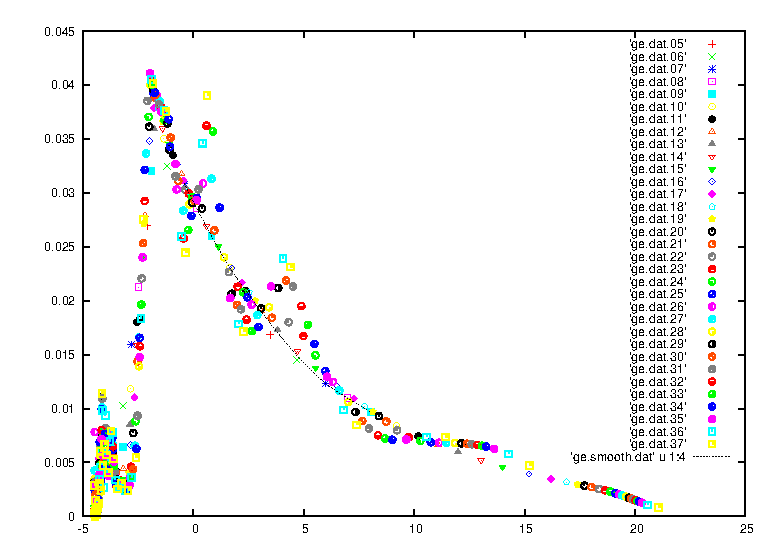
\includegraphics[scale=1.15]{pics/Xe4p_33_gammae.eps}
  \caption{Shifted Stieltjes profile of $\Gamma(E)$ obtained from the
           relativistic FanoADC calculation from
           a 4p$_{3/2}$
           initial state with both $\Gamma$ and $E$ given in atomic units.
           The resonance energy is $E_{res}=0$ and the resulting points
           of the different orders of Stieltjes are plotted separately.
           The smooth curve shows two
           additional peaks realted to interactions with Rydberg states as
           discussed in section \ref{section:Stieltjes_profile_properties}.
           }
  \label{figure:Xe4p33_Gamma_profile}
\end{figure}

In case of a 4p$_{3/2}$ initial state, the decay width profile for Stieltjes
orders between 5 and 37 shows a decay
with a threshold at energies below $E_{ref}=0$, which leads to a fairly smooth
curve at the energy of interest.
At higher energies of about \unit[1.5]{a.u.} and
\unit[4.5]{a.u.} additional peaks are observed, which can be explained with
interactions of the initial state description with Rydberg states. These do not
contribute to the decay and hence a smoothing of the total curve neglecting them
is necessary.


\begin{table}[h]
 \centering
 \caption{Auger decay widths of the Xe4p$_{3/2}$ initial states with
          different $M_J$ values and different doubly ionized final
          states.
          All widths are given in \unit{eV}.}
 \begin{tabular}{lcc}
   \toprule
                      & 4p$_{3/2,\pm 3/2}$ & 4p$_{3/2,\pm 1/2}$  \\
   \midrule                                                      
   energy [\unit{eV}] &   147.57           &    147.57          \\
   pole strength       &     0.694          &      0.694         \\
   \midrule                                                     
   $4d^{-2}$          &      --            &        --            \\
   $4d^{-1}5s^{-1}$   & 1.31$\cdot10^{-1}$ & 1.44$\cdot10^{-1}$ \\
   $4d^{-1}5p^{-1}$   & 6.36$\cdot10^{-1}$ & 6.29$\cdot10^{-1}$ \\
   $5s^{-2}$          & 6.27$\cdot10^{-4}$ & 6.29$\cdot10^{-4}$ \\
   $5s^{-1}5p^{-1}$   & 1.50$\cdot10^{-2}$ & 1.49$\cdot10^{-2}$ \\
   $5p^{-1}5p^{-1}$   & 3.21$\cdot10^{-2}$ & 2.90$\cdot10^{-2}$ \\
   \midrule
   total              &   0.814            &   0.818            \\
   \bottomrule
 \end{tabular}
 \label{table:xe_auger_rest}
\end{table}


\begin{table}[]
 \centering
 \caption{Total Auger decay widths of the Xe4p$_{3/2}$ obtained from
          experiment, \ac{MCDF} and this work. All widths are given in \unit{eV}.}
 \begin{tabular}{lcccc}
   \toprule
                        & exp   & calc\footnotemark[1] & calc\footnotemark[2] & calc\footnotemark[3] \\
   \midrule                                                                         
   energy [\unit{eV}]   & 145.6 &  145.0       &  145.0       &   147.57   \\
   $\Gamma$ [\unit{eV}] &  0.54 &  1.80        &  0.3116      &  0.814\\
   \bottomrule
 \end{tabular}
 \label{table:xe_auger_comp}
\end{table}
\footnotetext[1]{\ac{MCDF} calculation excluding final ionic state configuration
                 interaction. \cite{Heinaesmaeki04}}
\footnotetext[2]{\ac{MCDF} calculation including final ionic state configuration
                 interaction. \cite{Heinaesmaeki04}}
\footnotetext[3]{This work.}

The total and partial decay widths for the 4p$_{3/2}$ initial state
are shown in Table \ref{table:xe_auger_rest}. The projection of the
angular total angular momentum of the initial state does not influence
the results, which can be deduced from the almost equal results for the
4p$_{3/2,\pm 3/2}$ and 4p$_{3/2,\pm 1/2}$ initial state. It can easily be seen that
the \ac{CK} processes characterized by the 4d$^{-1}$5s$^{-1}$ and
4d$^{-1}$5p$^{-1}$ final states dominate the decay.

The total decay widths are compared
to experimental values and the results obtained using \ac{MCDF} in
Table \ref{table:xe_auger_comp}. All decay widths are in the order of \unit[1]{eV}.
While the calculation excluding the final ionic state configuration interaction
underestimates
the experimental decay width by \unit[0.23]{eV}, the calculation including the
final ionic state configuration interaction overestimates the experimental value
by \unit[1.26]{eV}. 
The decay width obtained in this work overestimates the experimental decay width
by \unit[0.27]{eV}. 
The FanoADC-Stieltjes approach intrinsically contains configuration interaction
inside the final state subspace. However, only those states characterized by
certain 2h configurations imaging the final state configuration are taken
into account. In contrast to this, in the \ac{MCDF} calculation further hand-picked
satellite contributions are added to the final state description.
Hence, the final state description of the \ac{MCDF} can be more precise
than the one of the FanoADC method.

Considering the large errors of both decay width calculations
their experimental determination, the total decay widths
obtained in this work are in agreement with both the experimental findings and
the other calculations.

\begin{table}[]
  \centering
  \caption{Contributions of the different channels to the total
           decay width for the Auger decay of Xe4p$_{3/2}$ in \%.}
  \begin{tabular}{lccccc}
   \toprule
                   & 4d$^{-1}$5s$^{-1}$ & 4d$^{-1}$5p$^{-1}$ & 5s$^{-2}$ & 5s$^{-1}$5p$^{-1}$ & 5p$^{-2}$ \\
   \midrule
   Ref. \cite{Heinaesmaeki04}\footnotemark[1] & 77.7 & 20.7  &       0.5 &       --           & 1.1     \\
   Ref. \cite{Heinaesmaeki04}\footnotemark[2] & 33.6 & 59.4  &       2.2 &       --           & 4.8     \\
   This work       &      16.1          &       78.1         &    0.1    &     1.8            & 3.9    \\
   \bottomrule
  \end{tabular}
  \label{table:Xe_auger_distr}
\end{table}
%\footnotetext[1]{\ac{MCDF} calculation excluding final ionic state configuration
%                 interaction. \cite{Heinaesmaeki04}}
%\footnotetext[2]{\ac{MCDF} calculation including final ionic state configuration
%                 interaction. \cite{Heinaesmaeki04}}

As discussed in section \ref{section:partial}, the obtained partial decay
widths might suffer from interchannel mixing, which is mainly observed in
the subvalence region. According to this, the intensity distribution
of this work is differs from the ones of reference \cite{Heinaesmaeki04} as
shown in Table \ref{table:Xe_auger_distr}. However, the dominance of the
\ac{CK} process is qualitatively observed in accordance with the other
calculations.


The Xe4p$_{1/2}$ initial state can, as already mentioned, not be described
by a single 1h configuration and therefore, all states with a pole strength
larger than 0.05 and a major contribution of the Xe4p$_{1/2}$ spinor are
investigated. Hereby, also the $4d^{-2}$ configurations are sorted into the
final state subspace in order to take into account a possible \ac{SCK} process.

Figure \ref{figure:Xe4p11_Gamma_profile} shows the decay width profile
of the lowest energy state investigated, which also inhabits the largest
pole strength. It is a well-behaved and smooth curve at energies above $E=0$.
As can easily be seen, the \ac{SCK} decay channel opens directly
in the energy region of interest at $E_{res}=0$. Since the Stieltjes procedure
is not able to produce a clear energy cut at the threshold and the initial state
energies can be expected not to be completely exact due to errors introduced
by the partitioning and additional errors from the ADC(2x) itself, an
unambiguous conclusion, whether the \ac{SCK} channel is open or not, cannot be drawn.
This decission also determines the choice of which curve of the decay width
profile to choose for the evaluation of the decay width. The results shown
in Table \ref{table:xe_auger_rel11} are the numbers obtained from the
lower curve excluding
the opening channel from the interpolation. In weighing the higher order moments
more than the lower order moments, the decay width would be about twice
as large as the numbers
presented and hence in the order of $\Gamma_{max} \approx \unit[2]{eV}$.

\begin{figure}[]
  \centering
  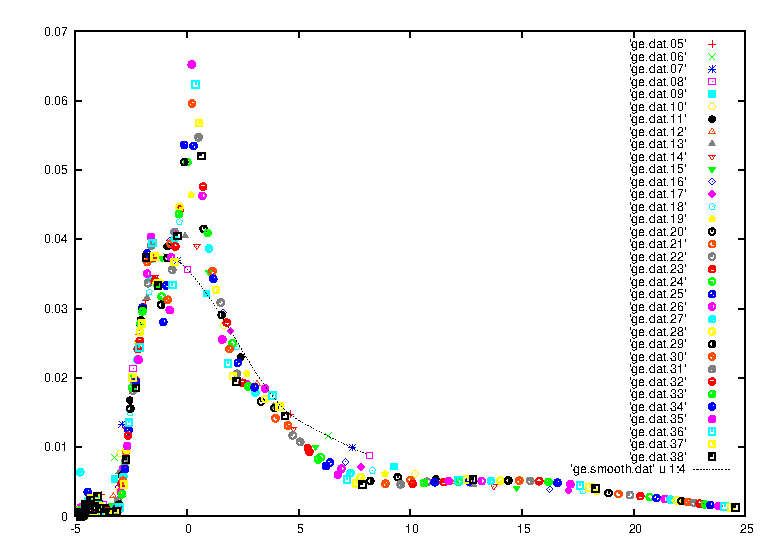
\includegraphics[scale=1.0]{pics/Xe4p_11_gammae.eps}
  \caption{$\Gamma(E)$ of the relativistic FanoADC calculation from a 4p$_{1/2}$
           initial state with both $\Gamma$ and $E$ given in atomic units.
           }
  \label{figure:Xe4p11_Gamma_profile}
\end{figure}


\begin{table}[]
 \centering
 \caption{Auger decay widths of non-negligible satellites with a major
          contribution of the Xe 4p$_{1/2}$. All widths are given in \unit{eV}.}
 \begin{tabular}{lccccc}
   \toprule
   energy [\unit{eV}] & 156.42  & 158.16 & 160.22 & 177.77 & 186.31\\
   pole strength       &   0.332 &   0.093&   0.123&   0.058&   0.068\\
   \midrule
   $4d^{-2}$          & 6.78$\cdot10^{-1}$ & 4.45$\cdot10^{-1}$ & 1.07$\cdot10^{-1}$ & 1.68$\cdot10^{-1}$ & 1.56$\cdot10^{-1}$\\
   $4d^{-1}5s^{-1}$   & 1.34$\cdot10^{-1}$ & 6.93$\cdot10^{-2}$ & 8.61$\cdot10^{-2}$ & 1.12$\cdot10^{-1}$ & 3.39$\cdot10^{-1}$\\
   $4d^{-1}5p^{-1}$   & 2.51$\cdot10^{-1}$ & 9.08$\cdot10^{-2}$ & 1.09$\cdot10^{-1}$ & 1.45$\cdot10^{-1}$ & 3.72$\cdot10^{-1}$\\
   $5s^{-2}$          & 3.10$\cdot10^{-4}$ & 2.21$\cdot10^{-4}$ & 1.91$\cdot10^{-4}$ & 2.12$\cdot10^{-4}$ & 1.81$\cdot10^{-4}$\\
   $5s^{-1}5p^{-1}$   & 3.84$\cdot10^{-3}$ & 1.32$\cdot10^{-3}$ & 2.16$\cdot10^{-3}$ & 1.45$\cdot10^{-3}$ & 8.13$\cdot10^{-3}$\\
   $5p^{-1}5p^{-1}$   & 1.02$\cdot10^{-2}$ & 3.40$\cdot10^{-3}$ & 5.12$\cdot10^{-3}$ & 2.18$\cdot10^{-3}$ & 1.55$\cdot10^{-2}$\\
   \midrule
   total              &   1.077 &   0.610&   0.310&   0.429&   0.891\\
   \bottomrule
 \end{tabular}
 \label{table:xe_auger_rel11}
\end{table}

Even though the FanoADC calculations imply the \ac{SCK} process to have
a large decay width, the calculated value is smaller than the estimated
value of \unit[10--100]{eV} \cite{Heinaesmaeki04}.
I therefore conclude that the broad
feature of the single ionization spectrum in the 4p$_{1/2}$ region is caused
by both the breakdown of the single particle picture with additional fast decay
of all corresponding satellite configurations.


\section{Summary}
From these examples I have shown that the FanoADC-Stieltjes method implemented
in Dirac is able to both reproduce results of the comparable non-relativistic
code of Koloren\v{c}  and results from \ac{MCDF} calculations
including relativistic effects in Auger processes as well as the corresponding
experimental results.
It is to be expected that the relativistic FanoADC-Stieltjes Code is also able
to predict unknown decay widths for larger systems such as dimers and small
clusters, since it is able to treat lower than spherical symmetries.
